\documentclass[12pt,t]{beamer}
\usepackage{amsmath, graphicx, kbordermatrix,bm, animate,hyperref}


\usepackage{tikz}
\usetikzlibrary{positioning}

\setbeameroption{hide notes}
\setbeamertemplate{note page}[plain]



% page number
\setbeamertemplate{footline}{%
    \raisebox{5pt}{\makebox[\paperwidth]{\hfill\makebox[20pt]{\color{gray}
          \scriptsize\insertframenumber}}}\hspace*{5pt}}

% add a bit of space at the top of the notes page
\addtobeamertemplate{note page}{\setlength{\parskip}{12pt}}


% a few macros
\newcommand{\subt}[1]{{\footnotesize \color{subtitle} {#1}}}

% title info
\title{Machine Learning 101}
\author{\href{http://richcorrado.github.io}{Richard Corrado}}
\institute{Fat Cat Machine Learning}
\date{\href{https://github.com/richcorrado}{\tt \scriptsize github.com/richcorrado}}

\begin{document}

% title slide
{
	\setbeamertemplate{footline}{} % no page number here
	\frame{
		\titlepage
} } 
	


\begin{frame}{Goals}

\begin{itemize}
\item Summarize some types and examples of Machine Learning.
\item Examine details of parametric models and how to train them.
\item Motivate and discuss Neural Networks (NNs), including Convolutional and Recurrent NNs, along with some applications.
\end{itemize}


\end{frame}

\begin{frame}{Types of Machine Learning}

{\bf Supervised Learning} 
\bigskip

 Have a definite {\bf target} that we want to compute from observed {\bf features} of data.  
\bigskip

Ex:
\begin{itemize}
\item   Predict price of something.
\item  Does patient have some disease?
\item Image and facial recognition.
\end{itemize}


\end{frame}

\begin{frame}

{\bf Unsupervised Learning}
\bigskip

 Have data with  observed features,  but not a clear idea of what can be predicted. 
\bigskip

Approaches include:

\begin{itemize}
\item {\bf Clustering}: How do features segment data into groups of similar examples? Ex: Segment population into communites/market segments,  also genetic sequencing.
\item {\bf Anomaly Detection}: Are some examples considerably different from all of the rest? Ex: Fraud detection, network intrusion.  
\item {\bf Latent Variables}: Identify potential targets for supervised learning on data.

\end{itemize}
\end{frame}

\begin{frame}

{\bf Reinforcement Learning}: 
\bigskip

Train {\bf software agent} to take {\bf actions} in an {\bf enviroment} to maximize {\bf cumulative reward}.  
\bigskip

Ex:

\begin{itemize}
\item Game agents (AlphaGo),
\item Robot control (autonomous vehicles).
\end{itemize}
\end{frame}

\begin{frame}{Supervised Machine Learning}

From some quantities $\mathbf{x}$ (the {\bf features}), predict a value for a quantity $y$ (the {\bf target}).   In principle, there is some functional relationship
$$ y = f(\mathbf{x}).$$
However:
\begin{itemize}
\item Detailed form of $f$ is unknown (complexity of underlying system).
\item Predictors $\mathbf{x}$ may be incomplete or imperfect (complexity of data, randomness). Even if we knew $f$,  could only compute within some margin of error
$$ f(\mathbf{x}) = y \pm \epsilon.$$
\end{itemize}

\end{frame}

\begin{frame}

{\bf Machine Learning} (ML)  includes the study and application of algorithmic models to find approximations  
$$ \hat{f}(\mathbf{x} )\approx f(\mathbf{x}). $$
Statistical principles of validation, inference, etc., are used to determine the errors of the models.


\bigskip

{\bf Regression}: Target $y$ is a continuous variable.
\begin{itemize}
\item Prices or other expected values. 
\item Expected demand in number of units  (approximately continuous for large numbers).
\item Physical dimension of object (area, mass).
\end{itemize}

\end{frame}

\begin{frame}

{\bf Classification}: Target $y$ takes some discrete and finite number of values.

\begin{itemize}
\item What is the species of the object? (Iris classification)
\centerline{
\includegraphics[height=0.5\textheight]{./images/iris.png}
}  
\end{itemize}

\end{frame}

\begin{frame}
\begin{itemize}
\item Image recognition
\centerline{
\includegraphics[height=0.8\textheight]{./images/dogorbear.png}
} 
\end{itemize}

\end{frame}

\begin{frame}{Parametric Models} 

In many models $ \hat{f}(\mathbf{x} , \bm{\theta})$ depends on both the features $\mathbf{x}$ and some {\bf parameters} $\bm{\theta}$.
\bigskip

Examples:
\begin{itemize}
\item {\bf Linear models}:
\begin{equation*} \begin{split}
& \mathbf{x} = (x_1, \ldots, x_F), \\
& \bm{\theta}  = (\theta_0, \ldots, \theta_F), \\
& y = \bm{\theta} \cdot \mathbf{x} = \theta_0 +  \theta_1 x_1 + \cdots  \theta_F x_F.
\end{split} \end{equation*}

\item {\bf Generalized Linear models (GLMs)}:
\begin{equation*}y = \bm{\theta} \cdot \bm{g}( \mathbf{x} )= \theta_0 +  \theta_1 g_1( \mathbf{x} ) + \cdots  \theta_N g_N( \mathbf{x} ).
 \end{equation*}
\end{itemize}

\end{frame}

\begin{frame}{Training Parametric Models}

{\bf Statistical Intuition}: Want to maximize the probability that our model predicts the correct target: 
$$p(y|\mathbf{x}\bm{\theta} ) = \prod_i p(y_i|\mathbf{x}_i\bm{\theta} ) .$$
{\bf Technical point}: Maximizing this probability is equivalent to minimizing
$$  J(\bm{\theta}) = - \ln p(y|\mathbf{x}\bm{\theta} )  = - \sum_i \ln p(y_i|\mathbf{x}_i\bm{\theta} ).$$
This function is called the  {\bf cost/loss function}.  Exchaning the product for a sum is a useful computational simplification.
\bigskip

Given training data $\{ (\mathbf{x}_i, y_i)\}$, find values $\bm{\theta}$ that minimize $J(\bm{\theta})$.

\end{frame}

\begin{frame}
Example: If $y$ is a continuous response, assume that the errors between the true and predicted values
$$ \mathbf{\epsilon} =\mathbf{ y} - \hat{\mathbf{y}} $$
are normally distributed, then 
$$ p(y | \mathbf{ x} ) = \mathcal{N}(y; \hat{y}, \sigma^2)= \prod_i  \mathcal{N}( y_i; \hat{ y_i}, \sigma^2),$$
$$  \mathcal{N}(y_i; \hat{y}_i, \sigma^2) 
	= \frac{1}{(2\pi \sigma^2)^{1/2}} \exp \left( - \frac{1}{2\sigma^2} |y_i - \hat{y}_i |^2 \right).$$
Then
$$J(\bm{\theta}) = - \sum_i \ln p(y_i|\mathbf{x}_i\bm{\theta} ) \sim  \sum_i  |y_i - \hat{y}_i |^2$$
We recognize $J$ as the residual sum of squares.
\end{frame}

\begin{frame}{Gradient Descent}
Cost function is minimized when
$$ \nabla_{\bm{\theta}} J(\bm{\theta})  =0.$$
At general $\bm{\theta}$,  $ \nabla_{\bm{\theta}} J(\bm{\theta})  \neq 0$, but consider the shift
$$ \bm{\theta}' =\bm{\theta} - \alpha   \nabla_{\bm{\theta}} J(\bm{\theta})  .$$
where $\alpha > 0$ is a small number. Then by Taylor expansion
$$ J(\bm{\theta}') \approx J(\bm{\theta})  - \alpha  | \nabla_{\bm{\theta}} J(\bm{\theta})|^2 <  J(\bm{\theta}).$$
We have reduced the cost function by this change of parameters.

\end{frame}

\begin{frame}

{\bf Gradient descent algorithm}: 

\bigskip
{\bf while} $ J(\bm{\theta}) > \delta$: ~~~\# tolerance parameter $\delta >0$
 $~~~~~~~  \bm{\theta} =\bm{\theta} - \alpha   \nabla_{\bm{\theta}} J(\bm{\theta})$

\bigskip
$\alpha$ is usually called the {\bf learning rate}.

\centerline{
\includegraphics[height=0.65\textheight]{gradient_descent.png}
}
\end{frame}


\begin{frame}{Bias vs. Variance Tradeoff} 

In any ML problem must look out for:
\begin{itemize}
\item {\bf Bias or underfit} if our model is too simple to faithfully match the data.   Can also say that the model has a low {\bf capacity} to absorb the information in the training data.
\bigskip

 Ex: Using linear model when data is clearly nonlinear.

\bigskip 

\item {\bf Variance or overfit} if our model agrees so well with training data that it fails to generalize to new data.  Can say that the model has too much capacity and learns the training data too well.

\bigskip 
Ex: Using model with number of parameters that is very large compared to number of features, number of examples in training set.
\end{itemize}

\end{frame}

\begin{frame}

Ex: Polynomial regression on simulated data.

\centerline{
\includegraphics[height=0.9\textheight]{./images/biasvsvariance_code.png}
} 
\end{frame}

\begin{frame}

\centerline{
\includegraphics[height=1\textheight]{./images/biasvsvariance_fits.png}
} 

\end{frame}

\begin{frame}

\centerline{
\includegraphics[height=1\textheight]{./images/biasvsvariance_error.png}
} 

\end{frame}

\begin{frame}

For this data, the linear model
$$ y = \theta_0 +  \theta_1 x$$
is reasonable, but a generalized linear model 
$$ y = \theta_0 +  \theta_1 x + \theta_2 x^2 + \cdots \theta_N x^N, $$
with $ N = 4, \cdots, 7$ has better performance.

\end{frame}

\begin{frame}{Beyond Generalized Linear Models}

 When  we have many features and a large training set, it is time-consuming to find suitable functions $ \bm{g}( \mathbf{x} )$ to use in a generalized linear model.

\begin{itemize}
\item Must examine the relationship between each feature $x_i$ and the target $y$ and try to determine a suitable $g_a$.
\item Must also examine relationships between the features $x_i$, since the best $g_a$ might be multivariate $g(x_1, x_2,\ldots)$.
\end{itemize}

Note that we can think of the $g_a$ as a new set of features that are "engineered" from the original features $x_i$.

\bigskip
Neural networks (NNs) can be thought of as providing a set of algorithmic methods to learn {\bf new features}.  We hopefully trade expensive manual feature engineering for lower-cost computational  resources. 
\end{frame}

\begin{frame}{Neural Networks}


In order to keep the training process mathematically stable and computationally managable, NNs are based on fairly simple functions:
\begin{itemize}
\item Linear functions:
\begin{equation*} \begin{split}
&  \mathbf{z^{(i)}} = \mathbf{f}^{(i-1)} \mathbf{W}^{(i)} + \mathbf{b}^{(i)}, \\
&  \mathbf{W}^{(i)}: ~~\text{weights, with shape}~(F_{i_1}, F_i), \\
&   \mathbf{b}^{(i)}:~~~~\text{biases, with shape}~( F_i).
\end{split} \end{equation*}
\item Nonlinear functions, called {\bf activation functions}:
$$ \mathbf{f}^{(i)} = g^{(i)}(\mathbf{z}^{(i)}).$$
\end{itemize}
\end{frame}

\begin{frame}

A single layer of a neural network computes new features
$$ \mathbf{f}^{(i)} = g^{(i)} \Bigl(\mathbf{f}^{(i-1)} \mathbf{W}^{(i)} + \mathbf{b}^{(i)}\Bigr),$$
where $\mathbf{f}^{(i-1)}$ are the features output by the previous layer.   Terminology for the layers is:
\begin{itemize}
\item {\bf Input layer}: The first layer of the network is designed to simply load in the input features $\mathbf{X}$ present in the dataset.
\item {\bf Output layer}: The last layer is designed to produce an output that can be compared directly to the targets $\mathbf{y}$.
\item {\bf Hidden layers}: The layers in between compute the new features $\mathbf{f}^{(i)}$.  Not connected to input or output. \\
{\bf Width}: Number of new features of a single hidden layer. \\
{\bf Depth}: Total number of hidden layers in the network.  If depth is $\geq 3$ we can say that we have a {\bf deep neural network}.
\end{itemize}
\end{frame}


\begin{frame}{Single Hidden Layer}


\tikzset{%
  every neuron/.style={
    circle,
    draw,
    minimum size=1cm
  },
  neuron missing/.style={
    draw=none, 
    scale=4,
    text height=0.333cm,
    execute at begin node=\color{black}$\vdots$
  },
}

\begin{center}
\resizebox{7.0cm}{!}{
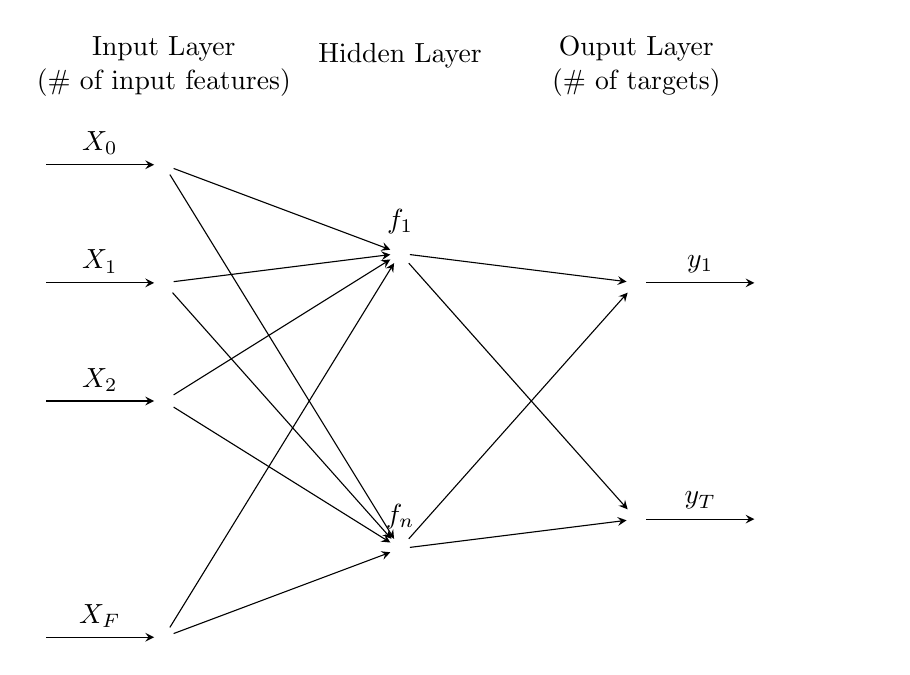
\begin{tikzpicture}[x=1.5cm, y=1.5cm, >=stealth]

\foreach \m/\l [count=\y] in {1,2,3,missing,4}
  \node [every neuron/.try, neuron \m/.try] (input-\m) at (0,2.5-\y) {};

\foreach \m [count=\y] in {1,missing,2}
  \node [every neuron/.try, neuron \m/.try ] (hidden-\m) at (2,2-\y*1.25) {};

\foreach \m [count=\y] in {1,missing,2}
  \node [every neuron/.try, neuron \m/.try ] (output-\m) at (4,1.5-\y) {};

\foreach \l [count=\i] in {0,1,2,F}
  \draw [<-] (input-\i) -- ++(-1,0)
    node [above, midway] {$X_\l$};

\foreach \l [count=\i] in {1,n}
  \node [above] at (hidden-\i.north) {$f_\l$};

\foreach \l [count=\i] in {1,T}
  \draw [->] (output-\i) -- ++(1,0)
    node [above, midway] {$y_\l$};

\foreach \i in {1,...,4}
  \foreach \j in {1,...,2}
    \draw [->] (input-\i) -- (hidden-\j);

\foreach \i in {1,...,2}
  \foreach \j in {1,...,2}
    \draw [->] (hidden-\i) -- (output-\j);

\foreach \l [count=\x from 0] in {Input Layer \\ (\# of input features), Hidden  Layer \\ \hfill, Ouput  Layer  \\ (\# of targets),}
  \node [align=center, above] at (\x*2,2) {\l };
\end{tikzpicture}
} \end{center}

A network like this, where every input feature is connected to a new feature is called a {\bf feedforward network} or, in older terms, a {\bf multilevel perceptron} (MLP).


\end{frame}

\begin{frame}{Composition of Functions}

Recall that a typical goal of machine learning is to approximate the functional relationship between the input features $\mathbf{X}$ and some target output $\mathbf{y}$:
$$ \mathbf{y} = f(\mathbf{X}) .$$
NNs naturally arrive at an approximation of this function via the composition of the functions learned at the hidden layers:
$$ \hat{f}(\mathbf{X}) = f^{(H)} \circ \cdots \circ f^{(1)}(\mathbf{X}).$$


\end{frame}

\begin{frame}{Activation Functions}

The activation functions  play a big role in allowing NNs to learning more general functions than linear models alone.  There are many possible choices, but the important characteristics are:
\begin{itemize}
\item {\bf Nonlinearity}: Key in allowing approximation of general functions, important for validity of {\bf universal approximation theorem}.
\item {\bf Differentiability}: Optimization of cost function uses {\bf backpropagation} through network to update weights and biases during training, need to have stable computations of gradients. 
\end{itemize}
Other characteristics like finite range, monotonicity, smoothness, etc., can be beneficial, but are not considered essential.  

\end{frame}

\begin{frame}{Rectified Linear Unit (ReLU)}
$$ g(z) = \text{max}(0,z) = \begin{cases} z, & z \geq 0 \\ 0, & z < 0. \end{cases}$$

\centerline{
\includegraphics[height=0.35\textheight]{./images/relu.png}
}

\begin{itemize}
\item {\bf Sparse Activation}: Negative inputs are set to zero.
\item {\bf Finite Gradients}: Differentiable on $\mathbb{R} {\char`\\} \{0\}$, with $g'(z) = 0, 1$.
\item Fast computations.
\end{itemize}

\end{frame}

\begin{frame}{Universal Approximation Theorem}

{\bf Theorem}: For a suitable choice of activation function, even a NN with a single hidden layer can approximate any function that we could reasonably expect to encounter in real-world machine learning problems (Borel measurable). 

{\bf Caveat}: The approximation error can be made arbitrarily small if the {\bf width} of the hidden layer is allowed to be {\bf arbitrarily large}. An arbitrarily wide NN will have {\bf many free parameters} and will be {\bf prone to overfitting} unless we also have an appropriately large and diverse training set.  

{\bf Deep Learning}: Add many hidden layers, learn larger classes of functions for smaller widths.

\end{frame}

\begin{frame}{Modifications of Feedforward Architecture}
In a fully-connected feed-forward network, each hidden layer feature is connected to a feature from the previous layer
$$ z_{a_i}^{(i)} = \sum_{a_{i-1}=0}^{F_{i-1}-1} f^{(i-1)}_{a_{i-1}} W_{a_{i-1} a_i}^{(i)} + b_{a_i}^{(i)}. $$
We can modify the rules for computing the new features, creating new {\bf architectures}, new types of NNs.

\begin{itemize}
\item[1.] We can force some of the weights  $\mathbf{W}^{(i)}_{a_{i-1}a_i}$ to zero.  This generally results in fully-connected models with a smaller capacity.
\centerline{
\includegraphics[height=0.2\textheight]{./images/dropout.png}
} 
\end{itemize}
\end{frame}

\begin{frame}
\begin{itemize}
\item[2.]  We can impose some symmetry on the weights $\mathbf{W}^{(i)}_{a_{i-1}a_i}$, forcing some components to be equal to one another. This is called {\bf weight sharing}.
\item[3.] We can remove some connections to the previous layer. This is equivalent to replacing 
$$ \mathbf{f}^{(i-1)} \mathbf{W}^{(i)} \rightarrow \sum_{a_{i-1} \in D} f^{(i-1)}_{a_{i-1}} W^{(i)}_{a_{i-1}a_i},$$
where $D$ is some subset of the index set for the incoming features $\mathbf{f}^{(i-1)}$. 
\centerline{
\includegraphics[height=0.4\textheight]{./images/semiconnect.png}
} 
\end{itemize}
\end{frame}

\begin{frame}
\begin{itemize}
\item[4.]  Can have more general connections between layers.
\begin{itemize}
\item {\bf Recurrent} networks have a chain structure between layers.

\centerline{
\includegraphics[height=0.4\textheight]{./images/recurrent.png} 
}
\item {\bf Recursive} networks have a tree structure.

\bigskip

\centerline{
\includegraphics[height=0.2\textheight]{./images/recursive.png}
} 
\end{itemize}
\end{itemize}

\end{frame}

\begin{frame}{Convolutional Neural Networks}

Convolutional NNs (CNNs) are designed to preserve information about how pixels in 2D images are spatially related:
\centerline{
\includegraphics[height=0.4\textheight]{./images/convolution.png} 
}
\begin{itemize}
\item {\bf  Partial connectivity}: Sample nearby pixels using a window.
\item {\bf Weight sharing}: Weights are shared over the whole image. 
\end{itemize}
\end{frame}

\begin{frame}

{\bf Filter}: Collection of weights forming a window.  Can use different filters to compute multiple types of features for a given image:

\centerline{
\includegraphics[height=0.4\textheight]{./images/filters.png} 
}

{\bf Translational invariance}: CNN filters tend to learn geometric shapes, regardless of where they appear in an image:

\centerline{
\includegraphics[height=0.3\textheight]{./images/convfeat.png} 
}

\end{frame}

\begin{frame}{Computer Vision}

Since CNNs are well-suited for processing 2D images (but can also be used for 3D and non-image problems),  they are extensively used in machine learning with images.

\begin{itemize}
\item {\bf Character recognition}: MNIST digits, zip codes:

\centerline{
\href{http://yann.lecun.com/exdb/lenet/gifs/asamples.gif}{\includegraphics[height=0.3\textheight]{./images/lenet-22.png}}
}
%\animategraphics[loop,controls,width=0.8\linewidth]{12}{./images/lenet-}{0}{30}
\end{itemize}
\end{frame}

\begin{frame}

Google Streetview: {\bf localization} and character recognition

\centerline{
\includegraphics[height=0.8\textheight]{./images/streetview.png} 
}

\end{frame}

\begin{frame}

ImageNet: {\bf object detection}

\centerline{
\includegraphics[height=0.8\textheight]{./images/imagenet-objdet.png} 
}

\end{frame}

\begin{frame}

ImageNet: {\bf classification}

\centerline{
\includegraphics[height=0.8\textheight]{./images/imagenet.png} 
}

\end{frame}

\begin{frame}

ImageNet: classification + {\bf localization}

\centerline{
\includegraphics[height=0.5\textheight]{./images/LocalizationDetection.png} 
}

\end{frame}





\begin{frame}{VGG-Network}
Simonyan and Zisserman,  ICLR 2015, arxiv:1409.1556,  1st/2nd in localization/classification, ImageNet ILSVRC-2014.

 \centerline{
\includegraphics[height=0.7\textheight]{./images/vgg19.png} 
}

\end{frame}



\begin{frame}{Recurrent Neural Nets}

Time-varying data: $ (\mathbf{X}_t, \mathbf{y}_t)  = \mathbf{s}_t \longrightarrow$ {\bf state} of system.

\bigskip

{\bf Causality}: state at time $\tau$, $\mathbf{s}_\tau$ must only depend on states at times $t<\tau$.

\bigskip

Dynamical system:
$$  \mathbf{s}_t = f( \mathbf{s}_{t-1}) = f(f( \mathbf{s}_{t-2})) = \cdots.$$

 \centerline{
\includegraphics[height=0.1\textheight]{./images/dynsys.png} 
}

\end{frame}

\begin{frame}{ Recurrent Neural Network to Approximate $f$}

\bigskip
Unfolded:
 \centerline{
\includegraphics[height=0.45\textheight]{./images/unfolded-rnn.png} 
}

\bigskip
Folded:
 \centerline{
\includegraphics[height=0.25\textheight]{./images/folded-rnn.png} 
}

\end{frame}

\begin{frame}{RNN Applications}

Important when sequential relationship is important.

\begin{itemize}
\item Time series:  stock price, weather,  resource demand
\item Language processing: word order $\rightarrow$ grammar, semantics \\
\hspace{1cm} spell/grammar-checking, translation 
\item Audio: speech recognition, signal processing/detection
\end{itemize}


\end{frame}

\begin{frame}
\begin{tabular}{ll}
For {\bf prediction}: &  train on $(x_{-n}, \cdots x_{-1})$, \\
& with targets $(x_{-n+1}, \cdots, x_0)$:
\end{tabular}

 \centerline{
\includegraphics[height=0.7\textheight]{./images/rnn-predict.png} 
}

\end{frame}

{\bf Credits:} \\
{\scriptsize
Several images and other graphics  in this presentation are reproduced as a fair use of the original sources:
\begin{itemize}
\item The original source of the photo used in the twitter post on page 9 appears to be \href{https://www.reddit.com/r/aww/comments/59zz7g/my_friends_new_pup_kuma/}{\color{blue} yamesjames@reddit}.
\item The image of the rectified linear unit is taken from \href{https://en.wikipedia.org/wiki/Ramp_function#/media/File:Ramp_function.svg}{\color{blue} wikimedia).
\item The graphic on page 33 was copied from the section of Yann LeCun's website on \href{http://yann.lecun.com/exdb/lenet/index.html}{\color{blue}LeNet-5}.
\item The image on page 34 was obtained from Goodfellow et al., \href{https://arxiv.org/abs/1312.6082}{\color{blue} arxiv:1312.6082}.
\item The image on page 35 was obtained from \href{http://www.image-net.org}{\color{blue} ImageNet}.
\item The image on page 36 is from \href{https://www.cs.toronto.edu/~kriz/imagenet_classification_with_deep_convolutional.pdf}{\color{blue} Krizhevsky et al., NIPS 2012}.
\item The image on page 37 is from Stanford CS231n  lecture slides, obtained here via \href{https://chaosmail.github.io/deeplearning/2016/10/22/intro-to-deep-learning-for-computer-vision/}{\color{blue} C.\ K\"orner}.
\item The figure on page 38 was obtained from slides for a \href{https://www.csie.ntu.edu.tw/~yvchen/f105-adl/doc/161103_ConvolutionalNN.pdf}{\color{blue} lecture by M.\ Chang} in the  \href{https://www.csie.ntu.edu.tw/~yvchen/f105-adl/index.html}{\color{blue} Applied Deep Learning} course by Y.\ Chen.
\end{itemize}
The original creators of the content highlighted and linked to have my thanks and appreciation. }



\end{document}